\section{Evaluación}

\subsection{Medida de Error}
\label{subsec:medida_error}

Tanto para el caso de la segmentación de los vídeos como la reconstrucción de los marcadores, se tiene los verdaderos marcadores generados en la secuencia, por lo que es necesario establecer una medida de error sobre la salida de los algoritmos. Se eligió aplicar una metodología basada en la distancia euclidiana promedio, entre los marcadores de ambos conjuntos \cite{humaneva} . 

Asumiendo que los conjuntos de datos de salida de algoritmos y ground truth, tienen sus cuadros sincronizados temporalmente, en un cuadro [f] dado se tienen $M$ marcadores en un conjunto $ \boldsymbol{x},\quad\{m_{i}(x)\},i=1,\ldots,M $ , donde $ m_{i}(x)\in{\mathbf{R}^{3}} $ ( o $ \mathbf{R}^{2} $ para el caso de las vistas de cámaras individuales), y $ \boldsymbol{\tilde{x}} $ es el conjunto ground truth con la misma cantidad $M$ de marcadores alineados con $\boldsymbol{x}$ (el $i$-esimo marcador de $\boldsymbol{x}$ se corresponde con el  $i$-esimo marcador de $\boldsymbol{\tilde{x}}$), se calcula la distancia como

\begin{equation}
D(\boldsymbol{x_{f}},\boldsymbol{\tilde{x_{f}}})=\frac{1}{M}\sum_{i=1}^{M} \|m_{i}^{[f]}(\boldsymbol{x})-m_{i}^{[f]}(\boldsymbol{\tilde{x}})\|
\label{error_vs_ground_basica}
\end{equation}

Sin embargo, el calculo debe ser modificado para contemplar para el caso en que la cantidad de marcadores a la salida del procesamiento es menor a $M$, se define un conjunto binario en cada frame $\Delta=\{\delta_1,\delta_2,\ldots,\delta_M\}$, donde $\delta_i$ indica con 1 si el $i$-esimo marcador de $\boldsymbol{\tilde{x}}$ fue detectado, 0 en caso contrario. La ecuación \ref{error_vs_ground_basica} queda entonces

\begin{equation}
D(\boldsymbol{x_{f}},\boldsymbol{\tilde{x_{f}}},\Delta_{f})=\frac{1}{\sum_{j=1}^{M} \delta_j} \sum_{i=1}^{M} \delta_i.\|m_{i}^{[f]}(\boldsymbol{x})-m_{i}^{[f]}(\boldsymbol{\tilde{x}})\|
\label{error_vs_ground_deteccion}
\end{equation}

En una secuencia con $F$ frames, la performance promedio es calculada como el promedio de los errores en cada frame,

\begin{equation}
\mu_{secuencia} = \frac{1}{F}\sum_{f=1}^{F} D(\boldsymbol{x_{f}},\boldsymbol{\tilde{x_{f}}},\Delta_{f})
\label{performance_secuencia}
\end{equation}

Para poder trabajar con los datos a la salida de la segmentación y reconstrucción de las secuencias, es necesario obtener datos adicionales y entonces aplicar la ecuación \ref{performance_secuencia}. Específicamente, las parejas entre marcadores obtenidos y aquellos en el ground truth , que permite alinear y comparar los marcadores, y definir cuales fueron detectados.

El emparejamiento es realizado frame a frame, calculando en una matriz la distancia euclidiana entre todos los pares $\{i,j\}$, donde $i=1,\ldots,M_{x}$ es un marcador del conjunto $\boldsymbol{x}$ obtenido mediante algoritmo en un frame [f], y $j=1,\ldots,M_{\tilde{x}}$ es un marcador del conjunto $\boldsymbol{\tilde{x}}$ de ground truth,

\begin{equation}
d_{i,j}^{[f]} = \{\|m_{i}^{[f]}(\boldsymbol{x})-|m_{j}^{[f]}(\boldsymbol{\tilde{x}})\|\}
\label{distancia_algoritmo_ground}
\end{equation}

Una vez calculadas todas las distancias para un frame, se buscan aquellas parejas que presenta la menor distancia, relevando la pareja $(i,j)$  para la cual se verifica. Una vez obtenida esta distancia, los marcadores $(i,j)$ quedan descartados de la matriz, volviendo a buscar la siguiente pareja con distancia mínima, hasta que ya no queden elementos para emparejar (lo cual sucede en caso que se generen menos marcadores que en el ground truth como puede suceder en segmentación, o si todos los marcadores de ground truth ya fueron emparejados y sobran marcadores, como sucede en reconstrucción). Trabajar con las parejas en todos los grames de la secuencia, es análogo a trabajar con la ecuación (\ref{error_vs_ground_deteccion}).

Para las medidas de los distintos bloques, se trabajará no solo con el promedio de error de secuencia, sino también con la magnitud que cumple que el 99\% de los puntos o marcadores, estén por debajo de esa magnitud. Se decidió elegir esta representación, en vez de la desviación estándar debido a que el error en la distancia no presenta una distribución gaussiana, sino euclidiana, donde todos los errores están entre cero e infinito (en este caso, no se tiene error infinito ya que los coeficientes binarios de detección se anulan), donde el error promedio es aquel percentíl que la mayoría de los puntos está situado, y el 99\% es afín al error máximo esperado.

\subsection{Performance}

\subsubsection{Capturas Sintéticas}

Las múltiples secuencias sintéticas generadas en Blender como fue establecido en la sección\label{seccion_Base_Datos_Sintetica} son ingresadas al sistema, utilizando los parámetros de calibración de las cámaras simuladas y los vídeos generados para las 17 cámaras. Cada conjunto de datos fue procesado por cada uno de los bloques establecidos en la sección~\ref{sec:implementacion_bloques_sistema} y comparado con el ground truth obtenido por Blender junto a los vídeos utilizando la metodología establecida en la sección~\ref{subsec:medida_error} para medir los resultados a la salida de cada bloque. Se realizaron las pruebas para 5 secuencias, 2 de las cuales fueron probadas con distinta adquisición, indicadas en la tabla \ref{resultados_distintas_capturas} como $X,YY,Z$ donde $Z=1,2$ corresponden a dos tasas de muestreo diferentes.

\begin{table}[h]
\centering
\begin{tabular}{cccc|c|c|c|c|c|c|ll}
\cline{5-10}
& & & & SEGM. & SEGM. & RECONS. & RECONS. & TRACK. & TRACK. &  &  \\ \cline{1-10}
\multicolumn{1}{|c|}{captura} & \multicolumn{1}{c|}{markers} & \multicolumn{1}{c|}{frames} & n.cams & \begin{tabular}[c]{@{}c@{}}Promedio\\ (px)\end{tabular} & \begin{tabular}[c]{@{}c@{}}99\%\\ (px)\end{tabular} & \begin{tabular}[c]{@{}c@{}}Promedio\\ (cm)\end{tabular} & \begin{tabular}[c]{@{}c@{}}99\%\\ (cm)\end{tabular} & \begin{tabular}[c]{@{}c@{}}Promedio\\ (cm)\end{tabular} & \begin{tabular}[c]{@{}c@{}}99\%\\ (cm)\end{tabular} &  &  \\ \cline{1-10}
\multicolumn{1}{|c|}{8,03,1}  & \multicolumn{1}{c|}{14}         & \multicolumn{1}{c|}{89}     & 17      & 1,1063 & 3,6783  & 0,40778     & 2,6384  & 0,4318 & 2,9039  &  &  \\ \cline{1-10}
\multicolumn{1}{|c|}{8,07,1}  & \multicolumn{1}{c|}{14}         & \multicolumn{1}{c|}{62}     & 17      & 1,0871 & 3,1172  & 0,34382     & 1,806   & 0,34451     & 1,806   &  &  \\ \cline{1-10}
\multicolumn{1}{|c|}{8,07,2}  & \multicolumn{1}{c|}{14}         & \multicolumn{1}{c|}{123}    & 17      & 1,0912 & 3,3097  & 0,38736     & 1,2681
& 0,36381     & 1,2681  &  &  \\ \cline{1-10}
\multicolumn{1}{|c|}{8,11}    & \multicolumn{1}{c|}{13}         & \multicolumn{1}{c|}{94}     & 17      & 1,074  & 2,9042  & 0,38836     & 2,8705  & 0,38836     & 2,8705  &  &  \\ \cline{1-10}
\multicolumn{1}{|c|}{9,07,1}  & \multicolumn{1}{c|}{14}         & \multicolumn{1}{c|}{29}     & 17      & 1,1285 & 3,3211  & 0,28016     & 2,0401  & 0,28016     & 2,0401  &  &  \\ \cline{1-10}
\multicolumn{1}{|c|}{9,07,2}  & \multicolumn{1}{c|}{14}         & \multicolumn{1}{c|}{57}     & 17      & 1,1404 & 3,4476  & 0,34517     & 1,9902  & 0,34517     & 1,9902  &  &  \\ \cline{1-10}
\multicolumn{1}{|c|}{9,12,1}  & \multicolumn{1}{c|}{13}         & \multicolumn{1}{c|}{300}    & 15      & 1,0443 & 2,118   & 0,39731     & 1,4952  & 0,39741     & 1,4952  &  &  \\ \cline{1-10}
\end{tabular}
\caption{Resultados de los bloques, para distintas capturas sintéticas}
\label{resultados_distintas_capturas}
\end{table}

Los resultados para 17 cámaras arrojan resultados similares en distintas capturas para el caso de amplia disponibilidad de cámaras, y confirman los resultados y rendimientos presentados para los distintos bloques en las hipótesis planteadas para las capturas sintéticas. La segmentación de los vídeos presenta errores promedios alrededor del pixel y errores máximos del entorno de los 4 pixeles. La reconstrucción y el tracking presentan resultados similares, siendo la diferencia conceptual entre ambas el etiquetado de trayectorias, y presentan resultados con error medio menor a los 0.5 cm, y errores máximos por debajo de 5 cm para el caso de reconstrucción con 17 cámaras, y exceso de marcadores en reconstrucción (se establece como parámetro de puntos reconstruidos una cantidad mayor a la esperada) 

\subsubsection{Ruido En Segmentación}

La prueba consiste en relevar el error promedio en reconstrucción, contra el ground truth 3D para distintas instancias de información de múltiples vistas bajo ruido aleatorio de distintas magnitudes en pixeles en las coordenadas $X,Y$. Recordando que la diferencia entre las proyecciones 2D y los vídeos segmentados, son la visibilidad de los marcadores estimada en un 70\% por cámara y el error de segmentación estimada en 1 pixel, el ruido es inyectado entre la segmentación y la reconstrucción siendo evaluada la salida de reconstrucción contra el ground truth 3D con el procedimiento de la sección~\ref{subsec:medida_error} . En la tabla \ref{table_resolucion} de la sección\label{seccion_Base_Datos_Sintetica}, se estimo el impacto en metros del error en pixel cuya magnitud es relevada en el caso de la secuencia sintética.

\begin{table}[h]
\centering
\begin{tabular}{cc|c|c|c|c|c|c|}
\cline{3-8}
\textbf{} & \textbf{} & \multicolumn{2}{c|}{\textbf{\begin{tabular}[c]{@{}c@{}}14 marcadores\\ reconstruidos\end{tabular}}} & \multicolumn{2}{c|}{\textbf{\begin{tabular}[c]{@{}c@{}}18 marcadores\\ reconstruidos\end{tabular}}} & \multicolumn{2}{c|}{\textbf{\begin{tabular}[c]{@{}c@{}}30 marcadores\\ reconstruidos\end{tabular}}} \\ \hline
\multicolumn{1}{|c|}{\textbf{Conjunto}} & \textbf{\begin{tabular}[c]{@{}c@{}}Ruido\\ (pixels)\end{tabular}} & \textbf{\begin{tabular}[c]{@{}c@{}}Promedio\\ (cm)\end{tabular}} & \textbf{\begin{tabular}[c]{@{}c@{}}99\%\\ (cm)\end{tabular}} & \textbf{\begin{tabular}[c]{@{}c@{}}Promedio\\ (cm)\end{tabular}} & \textbf{\begin{tabular}[c]{@{}c@{}}99\%\\ (cm)\end{tabular}} & \textbf{\begin{tabular}[c]{@{}c@{}}Promedio\\ (cm)\end{tabular}} & \textbf{\begin{tabular}[c]{@{}c@{}}Promedio\\ (cm)\end{tabular}} \\ \hline
\multicolumn{1}{|c|}{Ground Cam} & 0 & 1,27E-10 & 1,01E-09 & 1,27E-10 & 1,01E-09 & 1,27E-10 & 1,01E-09 \\ \hline
\multicolumn{1}{|c|}{Segmentación} & 0 & 0,38553 & 1,6915 & 0,38553 & 1,6915 & 0,38305 & 1,6747 \\ \hline
\multicolumn{1}{|c|}{Ground Cam} & 0,5 & 1,0404 & 3,0757 & 0,5535 & 2,0504 & 0,53616 & 2,1104 \\ \hline
\multicolumn{1}{|c|}{Segmentación} & 0,5 & 0,76172 & 2,8548 & 0,70514 & 2,096 & 0,69771 & 2,0234 \\ \hline
\multicolumn{1}{|c|}{Ground Cam} & 1 & 1,6511 & 13,184 & 1,1398 & 5,1215 & 1,0356 & 3,7874 \\ \hline
\multicolumn{1}{|c|}{Segmentación} & 1 & 1,3948 & 9,2686 & 1,1158 & 3,8027 & 1,145 & 3,8481 \\ \hline
\multicolumn{1}{|c|}{Ground Cam} & 2 & 4,8746 & 59,8172 & 3,4818 & 53,3151 & 1,7094 & 7,4023 \\ \hline
\multicolumn{1}{|c|}{Segmentación} & 2 & 6,3302 & 49,8491 & 3,348 & 45,4941 & 2,0409 & 8,0023 \\ \hline
\multicolumn{1}{|c|}{Ground Cam} & 4 & 12,7279 & 131,2929 & 13,9006 & 121,5673 & 3,17 & 21,153 \\ \hline
\multicolumn{1}{|c|}{Segmentación} & 4 & 10,7759 & 67,2878 & 11,2504 & 102,6039 & 4,5432 & 40,5608 \\ \hline
\multicolumn{1}{|c|}{Ground Cam} & 8 & 22,6934 & 136,0204 & 21,8413 & 143,0939 & 8,7161 & 42,9549 \\ \hline
\multicolumn{1}{|c|}{Segmentación} & 8 & 25,7256 & 187,2483 & 24,2908 & 158,6828 & 8,6034 & 41,6941 \\ \hline
\end{tabular}
\caption{Resultados de Error en reconstrucción, para distintos caso de ruido agregado a la segmentación, tanto resultados sobre vídeos como sobre ground truth}
\end{table}

Las pruebas confirman los resultados estimados en \ref{table_resolucion} en la secuencia dada , con cámaras no alejadas mas de 10 metros del sujeto, hasta los 2 pixeles (recordar que el conjunto de segmentación ya ingresa un cierto error propio al cual se le agrega el ruido) el error promedio se mantiene en el orden de los pocos centímetros con instancias de error máximo mayores. Con el agregado que la reconstrucción es implementada con una cantidad variable de marcadores, la cual permite buscar de reconstruir una mayor cantidad de marcadores a los del sujeto para encontrar la mayor cantidad de posibilidades. A mayor cantidad de marcadores reconstruidos, se obtienen mejores resultados en los casos de mayor ruido.

\subsubsection{Variación Cantidad de Cámaras}

Hasta ahora todas las pruebas realizadas para los bloques presentados en la sección~\ref{sec:implementacion_bloques_sistema} , fueron realizadas sobre el conjunto entero de cámaras presentadas en la sección\label{seccion_Base_Datos_Sintetica}, con 17 puntos de vistas distintos en el espacio de captura de la figura \ref{img_espacio_capura}. Las pruebas de rendimiento con conjuntos reducidos de cámaras son realizadas sobre los últimos dos bloques de reconstrucción y tracking, debido a que no afectan el error en el bloque de segmentación, solo afecta la cantidad de videos para segmentar.

\begin{table}[h]
\centering
\begin{tabular}{|c|c|}
\hline
\textbf{CONJUNTO} & \textbf{CAMARAS} \\ \hline
C17 & 1,2,3,4,5,6,7,8,9,10,11,12,13,14,15,16,17 \\ \hline
C15 & 3,4,5,6,7,8,9,11,12,13,14,15,16,17 \\ \hline
C8 & 3,5,7,9,11,13,15,17 \\ \hline
C6.1 & 4,6,8,12,14,16 \\ \hline
C6.2 & 3,6,9,11,14,17 \\ \hline
C6.3 & 3,5,9,11,13,17 \\ \hline
C6.4 & 3,7,9,11,15,17 \\ \hline
C5.1 & 1,3,9,11,17 \\ \hline
C5.2 & 1,4,8,12,16 \\ \hline
C4.1 & 4,8,12,16 \\ \hline
C4.2 & 3,9,11,17 \\ \hline
\end{tabular}
\caption{Distintas Combinaciones de Amaras del laboratorio sintético, numeradas según la figura \ref{img_espacio_capura} presentada en la sección sección\label{seccion_Base_Datos_Sintetica} }
\end{table}

Las pruebas son realizadas sobre dos secuencias en particular, de distintas características de uso del espacio de captura de movimiento.

\paragraph{Captura de Marcha, Secuencia 8\_07\_100\_200}

En el movimiento de marcha de la captura 8\_07, muestreada al 200\% (48 frames por segundo), el sujeto se mueve en el espacio de captura desde el lugar de la figura \ref{img_espacio_capura} desde donde se encuentra la cámara 2 hasta donde está la cámara 10, caminando de forma rectilínea.

\begin{table}[h]
\centering
\begin{tabular}{c|c|c|c|c|c|}
\cline{2-6}
\textbf{} & \textbf{CONJUNTO} & \multicolumn{2}{c|}{\textbf{C17}} & \multicolumn{2}{c|}{\textbf{C8}} \\ \hline
\multicolumn{1}{|c|}{\textbf{MARKER}} & \textbf{NOMBRE} & \textbf{\begin{tabular}[c]{@{}c@{}}Promedio\\ (cm)\end{tabular}} & \textbf{\begin{tabular}[c]{@{}c@{}}99\%\\ (cm)\end{tabular}} & \textbf{\begin{tabular}[c]{@{}c@{}}Promedio\\ (cm)\end{tabular}} & \textbf{\begin{tabular}[c]{@{}c@{}}99\%\\ (cm)\end{tabular}} \\ \hline
\multicolumn{1}{|c|}{1} & LeftUpLeg & 0,3671 & 0,5158 & 0,3551 & 0,6197 \\ \hline
\multicolumn{1}{|c|}{2} & LeftLeg & 0,367 & 0,5411 & 0,3491 & 0,4464 \\ \hline
\multicolumn{1}{|c|}{3} & LeftFoot & 0,372 & 0,558 & 0,3582 & 0,5339 \\ \hline
\multicolumn{1}{|c|}{4} & RightUpLeg & 0,3714 & 0,5879 & 0,368 & 0,6825 \\ \hline
\multicolumn{1}{|c|}{5} & RightLeg & 0,378 & 0,586 & 0,3627 & 0,6065 \\ \hline
\multicolumn{1}{|c|}{6} & RightFoot & 0,4212 & 1,8483 & 0,3597 & 0,5667 \\ \hline
\multicolumn{1}{|c|}{7} & Spine & 0,404 & 0,6043 & 0,3819 & 0,5122 \\ \hline
\multicolumn{1}{|c|}{8} & Head & 0,3867 & 0,9063 & 0,3676 & 0,5208 \\ \hline
\multicolumn{1}{|c|}{9} & LeftArm & 0,3666 & 0,7997 & 0,3607 & 0,516 \\ \hline
\multicolumn{1}{|c|}{10} & LeftForeArm & 0,3873 & 0,9056 & 0,3621 & 0,6793 \\ \hline
\multicolumn{1}{|c|}{11} & LeftHand & 0,4007 & 1,1722 & 0,3667 & 0,7895 \\ \hline
\multicolumn{1}{|c|}{12} & RightArm & 0,4025 & 1,4771 & 0,3602 & 0,5078 \\ \hline
\multicolumn{1}{|c|}{13} & RightForeArm & 0,3844 & 0,781 & 0,36 & 0,5199 \\ \hline
\multicolumn{1}{|c|}{14} & RightHand & 0,3816 & 0,7728 & 0,3637 & 0,4884 \\ \hline
\multicolumn{1}{|c|}{\textbf{}} & \textbf{Secuencia} & \textbf{0,35686} & \textbf{0,81266} & \textbf{0,33603} & \textbf{0,53412} \\ \hline
\end{tabular}
\label{error_captura_marcha_17_8_camaras}
\caption{Error de Marcadores en Tracking para conjuntos de 17 y 8 cámaras en el caso de Marcha}
\end{table}

Con la máxima cantidad de cámaras, todos los marcadores son reconstruidos y sus trayectorias seguidas a lo largo de la secuencia, con las medidas de error ya encontradas hasta el momento, de error de marcador menor al centímetro, y errores máximos puntuales del orden de los pocos centímetros. Si se reduce el conjunto de cámaras, para tener una "visión doble" desde cada una de las esquinas en el espacio de captura, se mantiene el buen rendimiento del sistema, con errores similares a los obtenidos anteriormente,    obteniendo leves mejoras en algunos marcadores pero también leves incrementos en el error para otros, ambas situaciones equilibran el promedio de la secuencia. Ambos casos son presentados en la tabla \ref{error_captura_marcha_17_8_camaras} ,

\begin{table}[h]
\centering
\begin{tabular}{c|c|c|c|c|c|}
\cline{2-6}
\textbf{} & \textbf{CONJUNTO} & \multicolumn{2}{c|}{\textbf{C6.1}} & \multicolumn{2}{c|}{\textbf{C6.2}} \\ \hline
\multicolumn{1}{|c|}{\textbf{MARKER}} & \textbf{NOMBRE} & \textbf{\begin{tabular}[c]{@{}c@{}}Promedio\\ (cm)\end{tabular}} & \textbf{\begin{tabular}[c]{@{}c@{}}99\%\\ (cm)\end{tabular}} & \textbf{\begin{tabular}[c]{@{}c@{}}Promedio\\ (cm)\end{tabular}} & \textbf{\begin{tabular}[c]{@{}c@{}}99\%\\ cm)\end{tabular}} \\ \hline
\multicolumn{1}{|c|}{1} & LeftUpLeg & 5,821 & 37,6612 & 3,6182 & 45,3281 \\ \hline
\multicolumn{1}{|c|}{2} & LeftLeg & 0,3513 & 0,816 & PERDIDO & PERDIDO \\ \hline
\multicolumn{1}{|c|}{3} & LeftFoot & 0,3605 & 1,2945 & 0,3667 & 0,8624 \\ \hline
\multicolumn{1}{|c|}{4} & RightUpLeg & 4,1048 & 58,1895 & 1,2155 & 27,1109 \\ \hline
\multicolumn{1}{|c|}{5} & RightLeg & 0,3472 & 0,4227 & 0,3412 & 0,41 \\ \hline
\multicolumn{1}{|c|}{6} & RightFoot & 0,5627 & 9,3183 & 0,7806 & 19,5713 \\ \hline
\multicolumn{1}{|c|}{7} & Spine & 0,664 & 17,1032 & 0,4985 & 5,5806 \\ \hline
\multicolumn{1}{|c|}{8} & Head & 0,3559 & 0,4546 & 0,38 & 0,54 \\ \hline
\multicolumn{1}{|c|}{9} & LeftArm & 0,5959 & 6,4694 & 0,6544 & 9,2929 \\ \hline
\multicolumn{1}{|c|}{10} & LeftForeArm & 0,3472 & 0,4888 & 0,3608 & 0,656 \\ \hline
\multicolumn{1}{|c|}{11} & LeftHand & 0,3519 & 0,6833 & 0,3717 & 0,7004 \\ \hline
\multicolumn{1}{|c|}{12} & RightArm & 0,5879 & 6,7102 & 0,5145 & 9,4856 \\ \hline
\multicolumn{1}{|c|}{13} & RightForeArm & 0,3511 & 0,6307 & 0,3653 & 0,6726 \\ \hline
\multicolumn{1}{|c|}{14} & RightHand & 0,4799 & 7,4024 & 0,6051 & 14,0673 \\ \hline
 & \textbf{Secuencia} & \textbf{1,0095} & \textbf{24,3404} & \textbf{0,71806} & \textbf{17,1131} \\ \cline{2-6} 
\end{tabular}
\label{error_captura_marcha_61_62_camaras}
\caption{Error de Marcadores en Tracking para algunos conjuntos de 6 cámaras en el caso de Marcha}
\end{table}

Reduciendo el conjunto a 6 cámaras, comienza a influir no solo la cantidad sino la ubicación de las mismas. En la tabla \ref{error_captura_marcha_61_62_camaras} el conjunto 6.1 tiene 3 cámaras laterales sobre una misma pared en cada lado del "pasillo" donde camina el sujeto, y permite reconstruir la mitad de los marcadores sin problemas, pero la otra mitas presenta errores promedios altos, y picos de errores mas altos aún. El otro conjunto 6.2 presenta una distribución "hexagonal" rodeando al sujeto de captura, pero los resultados son similares al conjunto anterior.

\begin{table}[h]
\centering
\begin{tabular}{c|c|c|c|c|c|}
\cline{2-6}
\textbf{} & \textbf{CONJUNTO} & \multicolumn{2}{c|}{\textbf{C6.3}} & \multicolumn{2}{c|}{\textbf{C6.4}} \\ \hline
\multicolumn{1}{|c|}{\textbf{MARKER}} & \textbf{NOMBRE} & \textbf{\begin{tabular}[c]{@{}c@{}}Promedio\\ (cm)\end{tabular}} & \textbf{\begin{tabular}[c]{@{}c@{}}99\%\\ (cm)\end{tabular}} & \textbf{\begin{tabular}[c]{@{}c@{}}Promedio\\ (cm)\end{tabular}} & \textbf{\begin{tabular}[c]{@{}c@{}}99\%\\ (cm)\end{tabular}} \\ \hline
\multicolumn{1}{|c|}{1} & LeftUpLeg & 1,4455 & 22,4893 & PERDIDO & PERDIDO \\ \hline
\multicolumn{1}{|c|}{2} & LeftLeg & 0,3948 & 1,7799 & 0,5296 & 2,74 \\ \hline
\multicolumn{1}{|c|}{3} & LeftFoot & 0,3824 & 0,8816 & 0,3844 & 0,8658 \\ \hline
\multicolumn{1}{|c|}{4} & RightUpLeg & 1,1137 & 12,3685 & 1,4861 & 15,8273 \\ \hline
\multicolumn{1}{|c|}{5} & RightLeg & 0,4018 & 1,5785 & 0,3846 & 0,6913 \\ \hline
\multicolumn{1}{|c|}{6} & RightFoot & 0,3969 & 1,2771 & 0,393 & 1,3017 \\ \hline
\multicolumn{1}{|c|}{7} & Spine & 0,4152 & 1,4769 & 1,2313 & 10,2902 \\ \hline
\multicolumn{1}{|c|}{8} & Head & 0,384 & 0,7113 & 0,384 & 0,6934 \\ \hline
\multicolumn{1}{|c|}{9} & LeftArm & 0,5909 & 7,9405 & 0,3908 & 0,8389 \\ \hline
\multicolumn{1}{|c|}{10} & LeftForeArm & 0,4258 & 1,7149 & 0,3895 & 0,9638 \\ \hline
\multicolumn{1}{|c|}{11} & LeftHand & 0,3909 & 1,2141 & 0,3756 & 1,0439 \\ \hline
\multicolumn{1}{|c|}{12} & RightArm & 0,3756 & 0,7621 & 0,386 & 0,8189 \\ \hline
\multicolumn{1}{|c|}{13} & RightForeArm & 0,3968 & 0,9704 & 0,516 & 5,8124 \\ \hline
\multicolumn{1}{|c|}{14} & RightHand & 0,617 & 14,0623 & 0,7186 & 11,8042 \\ \hline
 & \textbf{Secuencia} & \textbf{0,51182} & \textbf{6,9322} & \textbf{0,5512} & \textbf{7,4726} \\ \cline{2-6} 
\end{tabular}
\label{error_captura_marcha_63_64_camaras}
\caption{Error de Marcadores en Tracking para algunos conjuntos alternativos de 6 cámaras en el caso de Marcha}
\end{table}

En la tabla \ref{error_captura_marcha_63_64_camaras}, se presentan los resultados de una combinación de cámaras usualmente ensayado en la bibliografía relevada ( \cite{gross2001cmu} , \cite{humaneva} ). El mismo consiste en no tener todas las cámaras especialmente distribuidas de forma similar como en el conjunto 6.1 o 6.2, sino tener un conjunto de 2 agrupadas y una tercer separada por cada lado, y cada lado tiene su conjunto de 2 cámaras del lado opuesto. Combinaciones de cámaras con esta geometría presentan resultados notoriamente mejores a las otras combinaciones de 6 cámaras ensayadas anteriormente.

Finalmente, los conjuntos de 5 cámaras ( Apéndice ,tabla \ref{error_captura_marcha_5_camaras} ) son solidarios a los conjuntos de 4 cámaras ( Apéndice tabla \ref{error_captura_marcha_4_camaras} ), donde solo los marcadores de los pies, hombros y cabeza logran buenos resultados. La única diferencia entre ambos conjuntos, es la cámara superior.

\paragraph{Captura de Movimiento Libre, 9\_12\_100\_100} 

La secuencia 9\_12 muestreada al 100\% (24fps), presenta un sujeto en movimiento libre caminando en círculos, hacia adelante y atrás en todo el espacio de captura. Debido a que en algunos momentos de la captura se perdían todos los marcadores en algunas cámaras (1, 2, 10) , y la reconstrucción no pueden procesar una cámara cuando no tiene marcadores en un momento dado, se decidió solo trabajar con las cámaras que tiene marcadores en todos los cuadros de la secuencia de 300 frames. Las trayectorias obtenidas en tracking y reconstrucción se observan en la figura \ref{captura_movimiento_libre} .

\begin{figure}[H]
  \centering
   \subfloat[Trayectorias Movimiento Libre.]{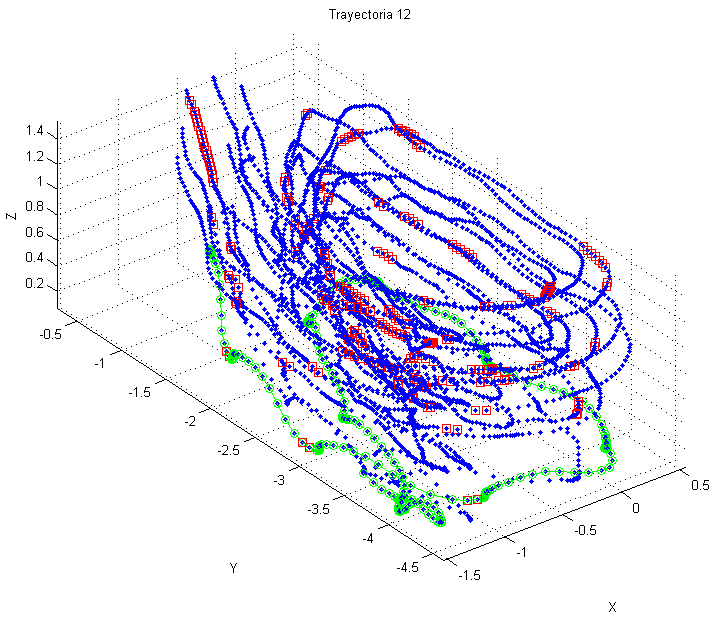
\includegraphics[scale=0.45]{img/Performance/00_Trayectorias_Tracking.png}\label{tracking_movimiento_libre}}\hspace{3 mm}
   \subfloat[Trayectoria Marcador, y Esqueleto reconstruido.]{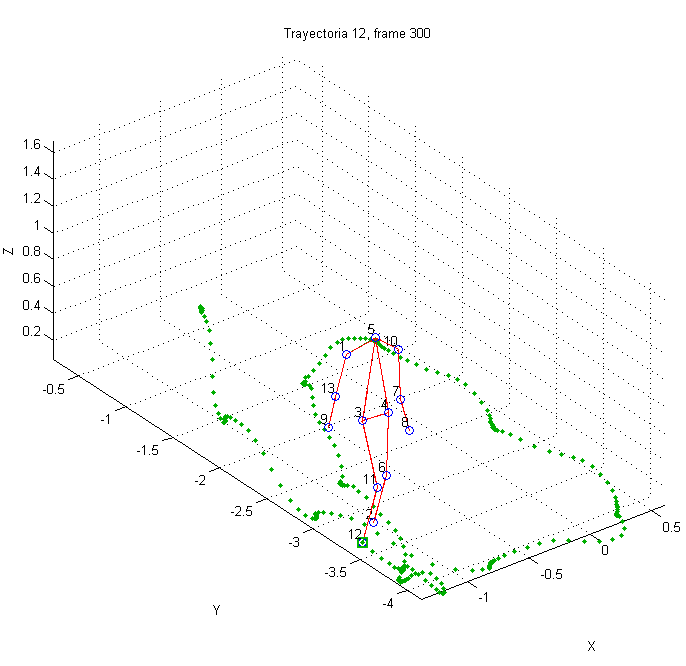
\includegraphics[scale=0.45]{img/Performance/00_Animacion_Tracking.png}}  
   \caption{Trayectorias obtenidas para Movimiento Libre.}
  \label{captura_movimiento_libre}
\end{figure} 

\begin{table}[h]
\centering
\begin{tabular}{c|c|c|c|c|c|}
\cline{2-6}
\textbf{} & \textbf{CONJUNTO} & \multicolumn{2}{c|}{\textbf{C15}} & \multicolumn{2}{c|}{\textbf{C8}} \\ \hline
\multicolumn{1}{|c|}{\textbf{NUMERO}} & \textbf{NOMBRE} & \textbf{\begin{tabular}[c]{@{}c@{}}Promedio\\ (cm)\end{tabular}} & \textbf{\begin{tabular}[c]{@{}c@{}}99\%\\ (cm)\end{tabular}} & \textbf{\begin{tabular}[c]{@{}c@{}}Promedio\\ (cm)\end{tabular}} & \textbf{\begin{tabular}[c]{@{}c@{}}99\%\\ (cm)\end{tabular}} \\ \hline
\multicolumn{1}{|c|}{1} & LeftUpLeg & 0,4695 & 2,7781 & 0,4232 & 1,2907 \\ \hline
\multicolumn{1}{|c|}{2} & LeftLeg & 0,4176 & 1,4028 & 0,4232 & 2,3317 \\ \hline
\multicolumn{1}{|c|}{3} & LeftFoot & 0,3935 & 0,714 & 0,4045 & 0,6123 \\ \hline
\multicolumn{1}{|c|}{4} & RightUpLeg & 0,4451 & 2,9214 & 0,3882 & 1,4679 \\ \hline
\multicolumn{1}{|c|}{5} & RightLeg & 0,3726 & 1,0633 & 0,3475 & 0,7875 \\ \hline
\multicolumn{1}{|c|}{6} & RightFoot & 0,3633 & 0,8745 & 0,3858 & 2,204 \\ \hline
\multicolumn{1}{|c|}{7} & Head & 0,4068 & 1,5204 & 0,369 & 0,5278 \\ \hline
\multicolumn{1}{|c|}{8} & LeftArm & 0,3951 & 0,7051 & 0,4139 & 1,4362 \\ \hline
\multicolumn{1}{|c|}{9} & LeftForeArm & 0,467 & 2,9049 & 0,3852 & 0,5232 \\ \hline
\multicolumn{1}{|c|}{10} & LeftHand & 0,4259 & 1,5519 & 0,3923 & 0,5664 \\ \hline
\multicolumn{1}{|c|}{11} & RightArm & 0,3845 & 0,8526 & 0,4395 & 1,7055 \\ \hline
\multicolumn{1}{|c|}{12} & RightForeArm & 0,3987 & 1,696 & 0,3441 & 0,5617 \\ \hline
\multicolumn{1}{|c|}{13} & RightHand & 0,3866 & 1,1216 & 0,3528 & 0,7263 \\ \hline
 & \textbf{Secuencia} & \textbf{0,39741} & \textbf{1,4952} & \textbf{0,37824} & \textbf{1,2867} \\ \cline{2-6} 
\end{tabular}
\label{error_captura_libre_15_8_camaras}
\caption{Error de Marcadores en Tracking para algunos conjuntos de 15 y 8 cámaras en el caso de Movimiento Libre}
\end{table}

Para el caso de todas las cámaras, o dos cámaras por esquina cuyos resultados son relevados en la tabla  \ref{error_captura_libre_15_8_camaras} , se confirman los resultados obtenidos en la captura de marcha de buenos resultados para todos los marcadores.

\begin{table}[h]
\centering
\begin{tabular}{c|c|c|c|c|c|}
\cline{2-6}
\textbf{} & \textbf{CONJUNTO} & \multicolumn{2}{c|}{\textbf{C6.3}} & \multicolumn{2}{c|}{\textbf{C4.2}} \\ \hline
\multicolumn{1}{|c|}{\textbf{NUMERO}} & \textbf{NOMBRE} & \textbf{\begin{tabular}[c]{@{}c@{}}Promedio\\ (cm)\end{tabular}} & \textbf{\begin{tabular}[c]{@{}c@{}}99\%\\ (cm)\end{tabular}} & \textbf{\begin{tabular}[c]{@{}c@{}}Promedio\\ (cm)\end{tabular}} & \textbf{\begin{tabular}[c]{@{}c@{}}99\%\\ (cm)\end{tabular}} \\ \hline
\multicolumn{1}{|c|}{1} & LeftUpLeg & 0,8081 & 9,8783 & 3,9761 & 23,5115 \\ \hline
\multicolumn{1}{|c|}{2} & LeftLeg & 0,5145 & 3,5296 & 0,959 & 9,4765 \\ \hline
\multicolumn{1}{|c|}{3} & LeftFoot & 0,4198 & 0,6535 & 0,9796 & 17,8756 \\ \hline
\multicolumn{1}{|c|}{4} & RightUpLeg & 0,4243 & 2,0492 & 6,5918 & 36,9034 \\ \hline
\multicolumn{1}{|c|}{5} & RightLeg & 0,3553 & 1,0051 & 0,8372 & 15,4254 \\ \hline
\multicolumn{1}{|c|}{6} & RightFoot & 0,3852 & 2,2009 & 1,1164 & 30,4735 \\ \hline
\multicolumn{1}{|c|}{7} & Head & 0,3803 & 0,5388 & 0,378 & 0,526 \\ \hline
\multicolumn{1}{|c|}{8} & LeftArm & 0,4288 & 1,3562 & 1,5435 & 20,0225 \\ \hline
\multicolumn{1}{|c|}{9} & LeftForeArm & 0,3955 & 0,5965 & 0,8621 & 12,847 \\ \hline
\multicolumn{1}{|c|}{10} & LeftHand & 0,398 & 0,5513 & 1,5922 & 17,1708 \\ \hline
\multicolumn{1}{|c|}{11} & RightArm & 0,5743 & 3,208 & 5,5887 & 25,7882 \\ \hline
\multicolumn{1}{|c|}{12} & RightForeArm & 0,358 & 0,6621 & PERDIDO & PERDIDO \\ \hline
\multicolumn{1}{|c|}{13} & RightHand & 0,3492 & 0,6748 & PERDIDO & PERDIDO \\ \hline
 & \textbf{Secuencia} & \textbf{0,43212} & \textbf{2,4391} & \textbf{1,8061} & \textbf{25,7332} \\ \cline{2-6} 
\end{tabular}
\label{error_captura_libre_6_4}
\caption{Error de Marcadores en Tracking para algunos conjuntos de 6 y 4 cámaras en el caso de Movimiento Libre}
\end{table}

Utilizando los conjuntos de 6 cámaras asimétricas lateralmente estudiado anteriormente, la tabla \ref{error_captura_libre_6_4} muestra que es posible tener un buen rendimiento para casi todos los marcadores. El único marcador con problemas, presenta un buen promedio de error pero un pico de error máximo a corregir. Finalmente el caso de 4 marcadores presenta malos resultados, con promedios aceptables, pero grandes errores máximos, y trayectorias que no se logran seguir en la totalidad de la secuencia.




